\section{Martyna Baran}




\subsection{WZÓR NEWTONA} 

Dla dowolej liczby całkowitej n oraz dla dowolnych liczb a i b:

\[(a+b)^n={n \choose 0}a^n + {n \choose 1}a^{(n-1)}b + ... + {n \choose k}a^{(n-k)}b^k + ... + {n \choose n-1}ab^{(n-1)} + {n \choose n}b^n \]


\begin{figure}[htbp]
\centering
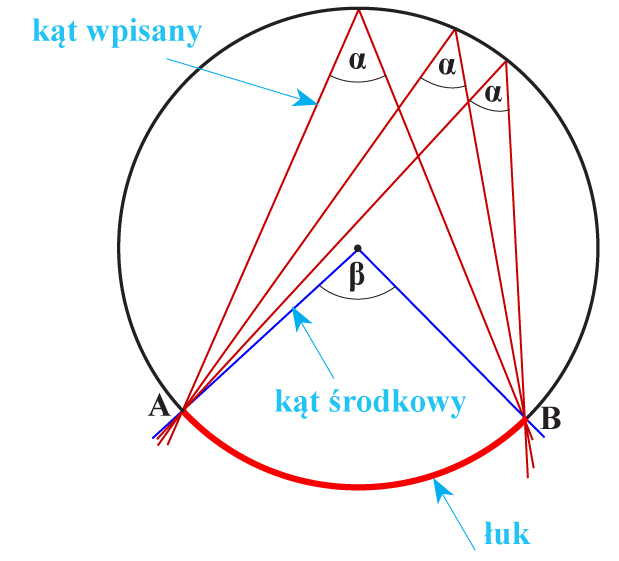
\includegraphics[width=0.6\textwidth]{pictures/katwpisany.jpg}
\caption{\label{fig: kąty wpisane}Kąty wpisane w okrąg}
\end{figure}


\begin{table}[h!]
\centering
\begin{tabular}{||c c c||} 
 \hline
 Lp. & Działanie & Skrót  \\ [0.5ex] 
 \hline\hline
 1. & Kopiuj & Ctrl+C  \\ 
 2. & Wklej & Ctrl+V  \\
 3. & Wytnij & Ctrl+X  \\
 4. & Zaznacz wszystko & Ctrl+A  \\ [1ex] 
 \hline
\end{tabular}
\caption{Skróty klawiszowe.}
\label{table:1}
\end{table}


\subsection{Lista numerowana i nienumerowana.}
\begin{enumerate}
  \item  The dollar has an exciting history. In 1520, the Kingdom of Bohemia began making coins using silver from a mine in Joachimsthal. 
  \item Logically, the coin was called the Joachimsthaler. Shortened to thaler the name found its way into other languages, for example, daler in Dutch.
  \item And, it was the Dutch coin that, thanks to booming international trade, made its way to the Dutch New Netherland Colony.

\end{enumerate}

\begin{itemize}
  \item[@]   It’s noteworthy that the modern pronunciation of dollar is remarkably close to the 17th-century Dutch pronunciation of daler. 
  \item[@]  Unfortunately, there is no straightforward answer to the question of how the dollar sign originated.
  \item[@] One theory is that the dollar sign comes from the Pillars of Hercules, as the Ancient Greeks used to call the two rocks at the entrance to the Straits of Gibraltar.
\end{itemize}




\begin{center}
HISTORY OF MYSTERIOUS KISS

"Immediately after President Truman announced Japan’s surrender in World War II,
at 7:03 p.m. on August 14, 1945, amid the crowds celebrating victory in Times Square,
\emph{ an American sailor shared a passionate kiss with a nurse who was passing by}. Or, at least,
that’s how the story went.

In fact, as reported by the New York Times in 2010, \textbf{Alfred Eisenstaedt’s famous photo
“The Kiss” might have been taken hours earlier}. Gloria Bullard, who was in Times Square that
day, claimed that \underline{she had seen the pair who were in the photograph kiss}. However, in her
eighties, when interviewed by the New York Times,\texttt{ she said that she had returned home on
August 14 by dusk.} As her house was 40 miles from Times Square, a long train ride away, she
can’t have been in New York as late as 7 p.m. "
\end{center}

odniesienie do zdjecia katów
\ref{fig: kąty wpisane}




